\subsection{GPR Results}

\lorena{By running GPR on the O2 testing dataset, we are able to better predict masses 
of the binary systems as shown in Fig.~\ref{m1_m2_chi_comparisons}.
The blue stars show the recovered values from the best-fit
template, the green dots are the predictions coming from regression, and the
true values are depicted by the red line. Ideally, all values would lie along 
the red line. The difference between the recovered and predicted values is 
clear especially in cases when the recovered masses are very high.  
Similarly, in Fig.~\ref{m_chi1_chi2_comparisons} the 
primary spins are closer to the true value using regression. Regression also
gets rid of highly negative and positive secondary spins that are far from the
true values. Although both the recovered and the predicted values have seemingly 
large errors, the predictions improve the overall error significantly.}

\begin{figure}
    \centering
    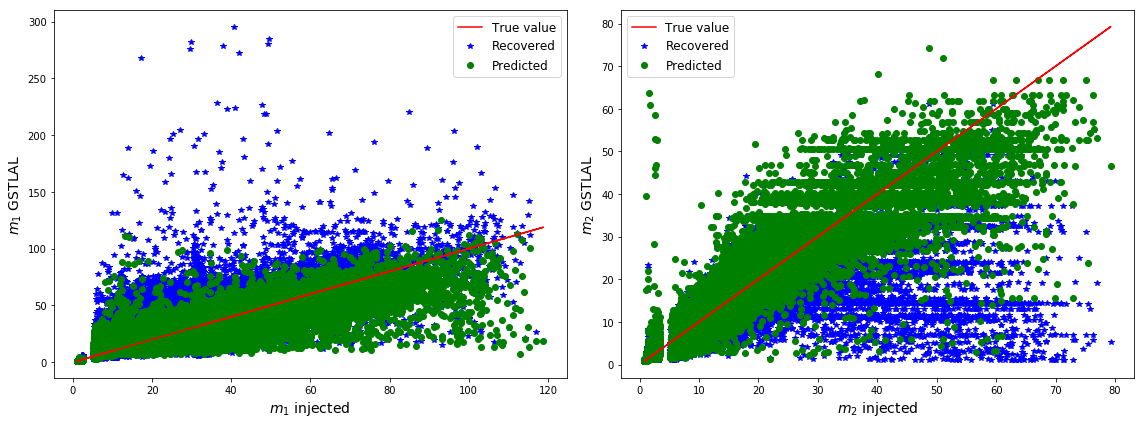
\includegraphics[width=0.45\textwidth]{m1_m2_chi_comparisons.png}
    \caption{\lorena{The recovered values are in blue, the predictions from
            regression are in green, and the true injected values are depicted
            by the red line for the $m_1$ values (left) and $m_2$ values
            (right).}}
        \label{m1_m2_chi_comparisons}
\end{figure}

\begin{figure}
    \centering
    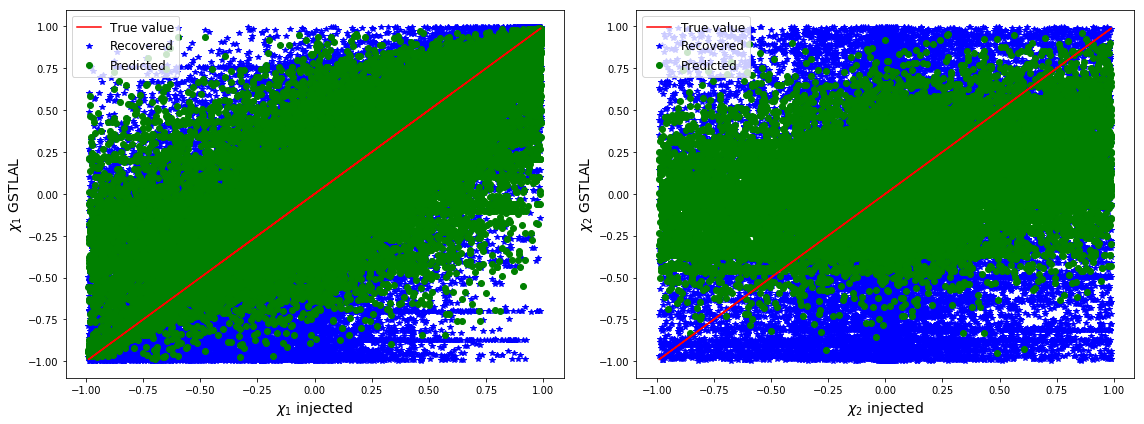
\includegraphics[width=0.45\textwidth]{m_chi1_chi2_comparisons.png}
    \caption{\lorena{The recovered values are in blue, the predictions from
            regression are in green, and the true injected values are depicted
            by the red line for the $\chi_1$ values (left) and $\chi_2$ values
            (right).}}
        \label{m_chi1_chi2_comparisons}
\end{figure}

\lorena{To quantify the above...}
